\documentclass[11pt, titlepage]{article}
\usepackage{amsmath,amsthm,amssymb}
\usepackage{hyperref, pgf, tikz}
\usepackage{fancyhdr}
\usetikzlibrary{arrows}
\usepackage[margin=1.25in]{geometry}
\usepackage{graphicx}                     
\pagestyle{fancy}
\usepackage{array}
%\usepackage{wrapfig}

\lhead{Lab \#6}
\rhead{\thepage}
\cfoot{}

\title{Conservation of Momentum in Explosions and Collisions\\ \ \\ \large Lab \#6}
\author{Name: Avery Karlin \\ Partner: Nicholas Yang}
\date{}
\begin{document}

\maketitle

\begin{center}
\LARGE Conservation of Momentum in Explosions and Collisions
\end{center}

\section*{Objective}
The objective is to measure the momentum of two carts before an explosion and after, to determine if momentum is conserved, and to observe the effects of a collision at varying velocities of both carts, both elastic and completely inelastic.

\section*{Introduction}
Conservation of momentum states that if there are no external forces acting on the body, then momentum is constant ($m_iv_i = m_1v_1 + m_2v_2$, in the case of an explosion). Thus, in an explosion, if the initial momentum was 0, $\frac{v_1}{v_2} = \frac{m_2}{m_1}$, and if the time of each body from the explosion is equal, $$\frac{x_1}{x_2} = \frac{m_2}{m_1}$$.

Similarly, this can apply to collisions, such that $$m_1v_{1i} + m_2v_{2i} = m_1v_{1f} + m_2v_{2f}.$$ Thus, in a completely inelastic collision where the bodies stick together, $$m_1v_{1i} + m_2v_{2i} = (m_1 + m_2)v_f.$$ In the case of elastic collisions, the equations hold true, but in addition, kinetic energy is conserved, such that $$\frac{1}{2}m_1v_{1i}^2 + \frac{1}{2}m_2v_{2i}^2 = \frac{1}{2}m_1v_{1f}^2 + \frac{1}{2}m_2v_{2f}^2.$$ 

\section*{Procedures and Results}
For this lab, after determining the mass of the cart, we placed the track flat on the table, testing to make sure it was level such that the carts didn't move, compressing the spring and placing them together. We then released the spring, such that they flew apart, and kept doing it until the time of collision with the end of the track was equal. After, we changed the mass of the carts and repeated the process.

For the next part of the lab, the carts began at either opposite sides or one at the end, one at the middle, turning the carts around, such that for elastic, the magnetic fields were repulsive, for completely inelastic, the magnetic fields were attractive, pushing with different amounts of initial velocity and mass to observe the effects of the collision under each of the cases.

\begin{figure}[p]
\centering
\hspace*{-10.5cm}
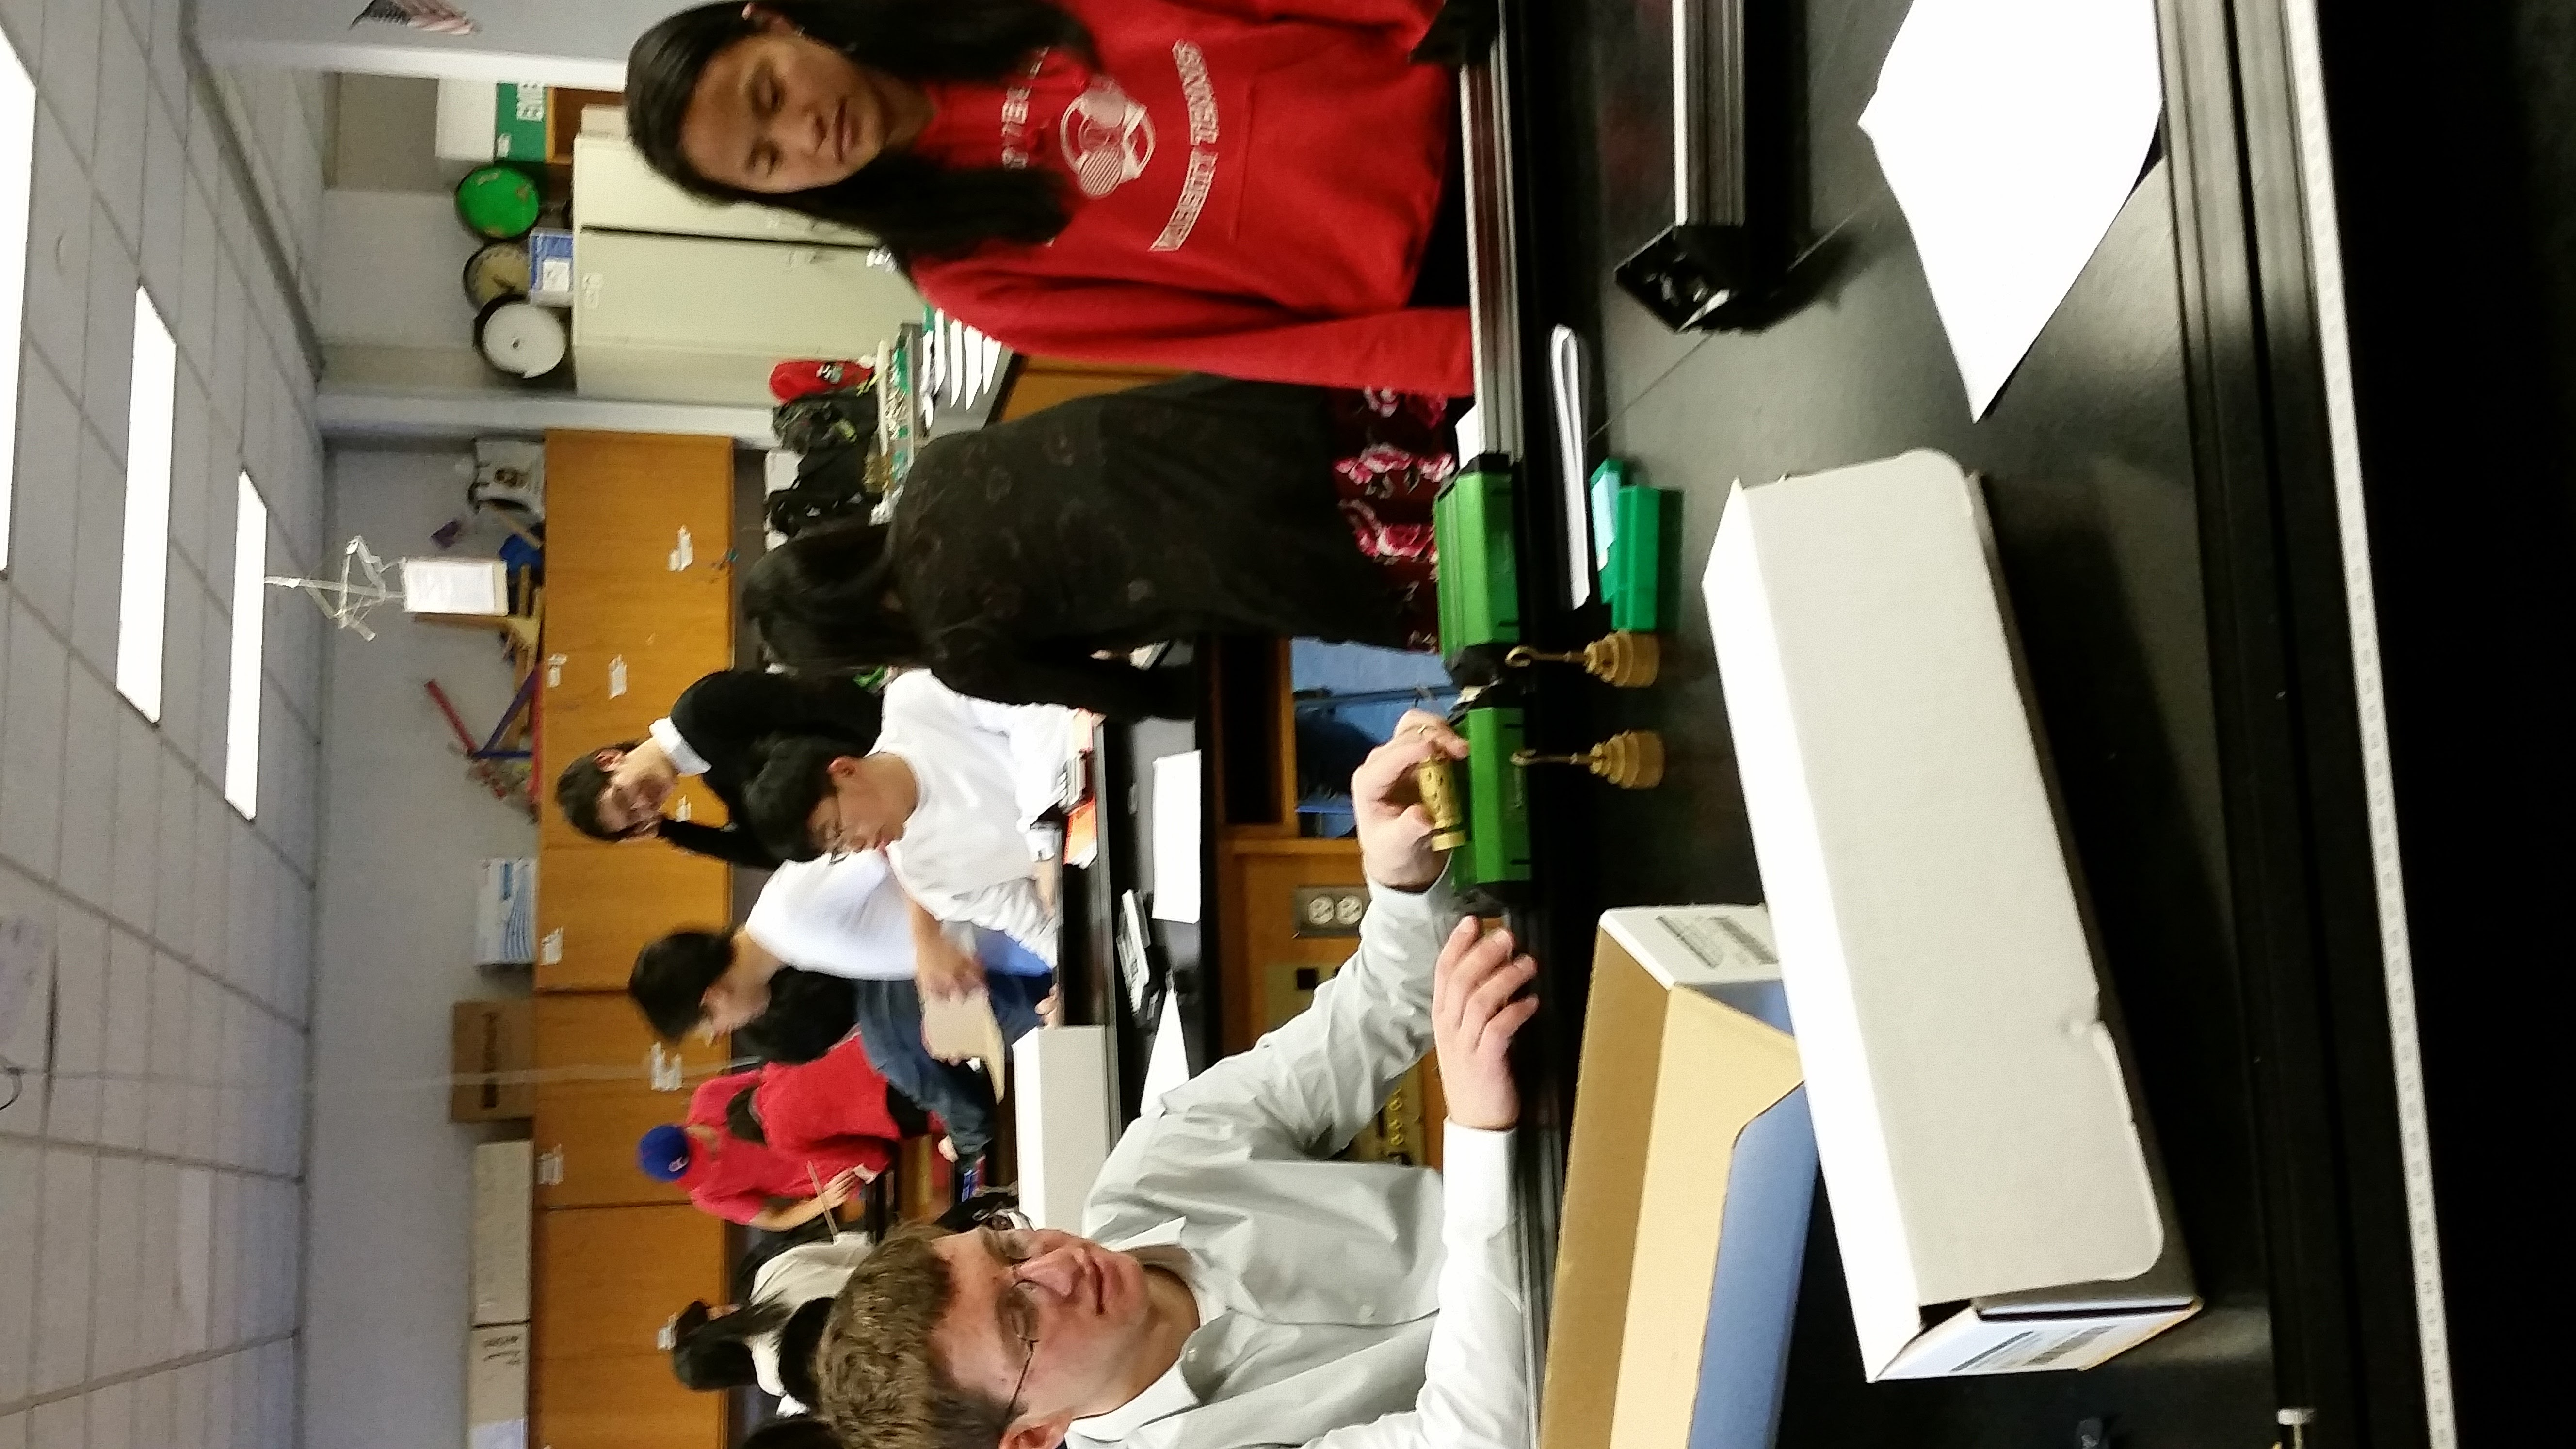
\includegraphics[scale=0.15, angle=270]{lab6.jpg}
\vspace*{19cm}
\end{figure}

\begin{center}
$$x_{left} = 0.05 m$$
$$x_{right} = 1.15 m$$
\begin{tabular}
{|m{7em}|m{7em}|m{7em}|m{7em}|m{7em}|}
\hline
Mass 1 (kg) & Mass 2 (kg) & Position (m) & $\Delta x_1$ & $\Delta x_2$ \\
\hline
0.5207 & 0.5187 & 0.62 & 0.53 & 0.57\\
\hline
0.7207 & 0.5187 & 0.65 & 0.5 & 0.6\\
\hline
0.9207 & 0.5187 & 0.715 & 0.435 & 0.665\\ 
\hline
0.9207 & 0.7187 & 0.64 & 0.51 & 0.59\\
\hline
\end{tabular}
\end{center}

\section*{Discussion}
Sample calculations for the non-measured data are as shown:
$$\frac{\Delta x_1}{\Delta x_2} \text{(Trial 1)} = \frac{0.53}{0.57} = 0.9298$$
$$\frac{m_2}{m_1} \text{(Trial 1)} = \frac{0.5187}{0.5207} = 0.996$$
$$\text{Percent Error} = \frac{|\frac{\Delta x_1}{\Delta x_2} - \frac{m_2}{m_1}|}{\frac{\Delta x_1}{\Delta x_2}} * 100\% = \frac{|0.9298 - 0.996|}{0.9296} * 100\% = 7.12\%$$

\begin{center}
\begin{tabular}
{|m{7em}|m{7em}|m{7em}|m{7em}|m{7em}|}
\hline
$\frac{\Delta x_1}{\Delta x_2}$ & $\frac{m_2}{m_1}$ & Percent Error \\
\hline
0.9298 & 0.996 & 7.12 \\
\hline
0.833 & 0.72 & 13.57 \\
\hline
0.654 & 0.563 & 13.9 \\
\hline
0.864 & 0.781 & 9.6 \\
\hline
\end{tabular}
\end{center}

Diagrams for Elastic and Inelastic Collisions
Credit to Kevin Yan
Cases A and B are elastic collisions, Cases C and D are completely inelastic collisions
\begin{figure}[p]
\centering
\hspace*{-7cm}
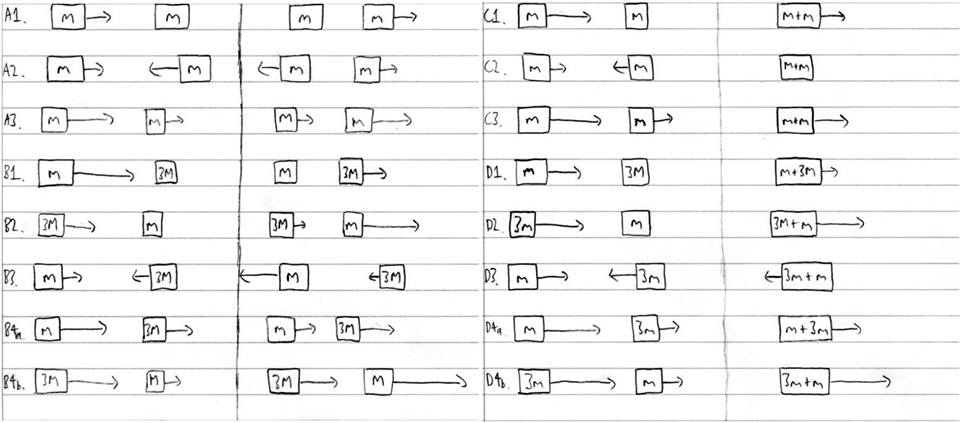
\includegraphics[scale=1, angle=270]{diagram6.jpg}
\vspace*{19cm}
\end{figure}

The most likely cause of percent error is the existance of external forces acting on the carts, in this case friction from the track, changing the total momentum of the system during travelling, as well as drag force doing the same. On the other hand, the percent error was fairly good, falling below 15\%, and half of the time below 10\%, showing the validity of conservation of momentum.

\section*{Conclusion}
The measured $\Delta x$ ratio for the test with equal masses was 0.9298, with a mass ratio of 0.996 for a percent error of 7.12\%. The measured $\Delta x$ ratio for the test with 0.2 kg added to one cart  was 0.833, with a mass ratio of 0.72 for a percent error of 13.57\%. The measured $\Delta x$ ratio for the test with 0.4 kg added to one cart was 0.654, with a mass ratio of 0.563 for a percent error of 13.9\%.The measured $\Delta x$ ratio for the test with 0.4 kg added to one cart, 0.2 kg added to the other was 0.864, with a mass ratio of 0.781 for a percent error of 9.6\%.

\end{document}
